\subsection{Teilversuch 3: Brewsterwinkel}

	\subsubsection*{Methoden}
		
		% TODO
		% soll bei dem aufgenommenen Wert zur glas reflexion als vergleich zur theorie in betracht genommen werden.
		
		\begin{figure}[ht]
			\centering
			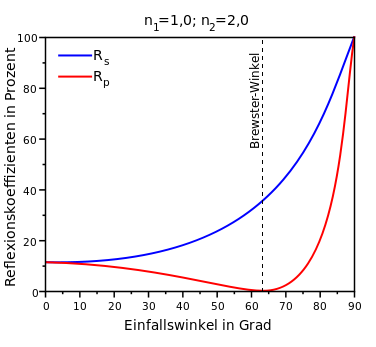
\includegraphics[width=\textwidth]{bilder/wikiBrewster.png}
			\caption{Theoretische Kurve des parallel polarisierten Anteils (rot, links) bei $n_2 = 2$. \cite{wikiBrewster}}
			\label{fig:wiki_brewster}	
		\end{figure}
				
		
	\subsubsection*{Durchführung}
	
		% TODO
	
	\subsubsection*{Datenanalyse}
		
		% TODO
	
	\subsubsection*{Diskussion}
	
		% TODO